\section{Notes of a Latter Day Knight}

\begin{quotex}
And it shall come to pass that I will pour out my spirit upon all flesh: and your sons and your daughters shall prophesy: your old men shall dream dreams, and your young men shall see visions. \flright{\textsc{Joel 2:28}}

\end{quotex}

\begin{wrapfigure}{rt}{.3\textwidth}
 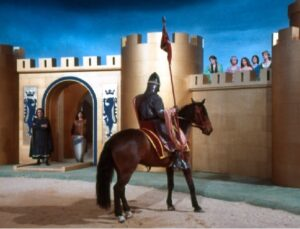
\includegraphics[scale=.5]{a20190313NotesofaLatterDayKnight-img001.jpg}
 \end{wrapfigure}

A knight is made, not born. He may have spent years like the prodigal son, living with the pigs, succumbing to Satan's three temptations of lust, the pride of life, and avarice. In our time, the knight of physical combat may not be necessary, but the knight of spiritual combat is needed more than ever.

\paragraph{Lady Love}
If he is fortunate, he may meet his Love, even if it is unrequited or even unknown. Such Love cannot be consummated carnally, the mistake made by Lancelot and Guinevere.

Her role is to send him on his quest. She chides him harshly when he falls short of the knightly ideal, through vulgarity, personal vanity, or pointless showmanship of his skills. Yet her gentleness inspires him to excel and to become a better man than he ever thought possible.

If you are fortunate, you will be able to see yourself through her eyes.

\paragraph{Duels}
\begin{quotex}
Whatever is acquired by single combat [duel] is acquired with Right. For when human judgment fails, either because it is wrapped in the darkness of ignorance or because it has not the aid of a judge, then, lest judgment should remain forsaken, recourse must be had to Him who so loved her that, by the shedding of His own blood, He met her full demands in death. Hence the Psalm: ``The righteous Lord loveth righteousness." This end is accomplished when, with the free consent of the participants, in love and not in hatred of justice, the judgment of God is sought through a mutual trial of bodily and spiritual strength. Because it was first used in single combat of man to man, this trial of strength we call the duel. \flright{\textsc{Dante, }\emph{De Monarchia}}

\end{quotex}
Combat can lead to the Truth, provided it is not motivated by rage, vengeance, or personal glory.

\paragraph{Initiation}
The \emph{Ordre de la Rose-Croix catholique et esthétique du Temple et du Graal}\footnote{\url{https://en.wikipedia.org/wiki/Salon_de_la_Rose_\%2B_Croix}}, founded by \textbf{Josephin Peladan}, consisted of three grades:

\begin{itemize}
\item \textbf{Neophyte} whose patron was \textbf{Leonardo da Vinci} 
\item \textbf{Chevalier} whose patron was \textbf{Dante} 
\item \textbf{Commander} whose patrons were \textbf{Saint John} and the Holy Spirit 
\end{itemize}
Dante the artist shows the Knight the stages of the journey to Sophia through the Divine Feminine, represented by Beatrice.

\paragraph{Judgment}
\begin{quotex}
Nobility, the quality which I call true aristocracy, requires of a man the recognition of his guilt. In its depths, conscience, which is frequently covered up and suppressed, is always a consciousness of guilt. The necessary thing is to take upon oneself as much guilt as possible and to put as little as possible of it upon other people. The aristocrat is not one who is proudly conscious of himself as first, as a privileged being, and who safeguards his position as such. The aristocrat is the man who is aware of the guilt and sinfulness of this first place, this privileged position of his. \emph{The sense that one is being continually affronted is on the other hand, precisely a plebeian feeling}. \flright{\textsc{Nicolai Berdyaev}} 

\end{quotex}
The knight knows his state of being and judges himself more harshly than any outsider could.

\paragraph{Motivation}
\begin{quotex}
From this deeper principle you must do your works, without a why. I affirm it decisively: even if you do your works for the kingdom of heaven, for God, or your sanctity, although motivated by the other, even then you will not really be in the right. If you ask a true man, a man who acts from his depth: ``Why do you do all your works?" he will answer you rightly only if he says: ``I act only for the action itself." \flright{\textsc{Meister Eckhart}}

\end{quotex}
The Knight follows his Dharma, or Destiny.

\paragraph{Anti-Realism}
\begin{quotex}
The truth or falsity of idealism—and that means if man can or can't give certainty and sense to his life and his experience—cannot be demonstrated theoretically: it can be decided not through an intellectual act, but through a concrete realization. \flright{\textsc{Julius Evola}, \emph{Essays on Magical Idealism}}

\end{quotex}
The animal mind cannot conceive of any reality beyond what appears to the senses. Yet, in the ascent to the divine, sensory images are left behind as one contemplates God and the Angels. Then the Knight returns to his Native Land, seeing through intuition, not the senses.

\paragraph{Intellectual Joy}
The animal mind believes that joy can arise only from sensory objects. Yet the greatest joy comes from intellectual pursuits. When I was a boy around 10 and 11, my parents sent me to weekly classes at the Boston Museum of Science. Afterwards, I would wait in the library to be picked up. My favourite topics were astronomy and mathematics. I learned the mystical symbols for the planets and constellations. I was fascinated with the ancient names of the stars like Aldebaran, Rigel, Betelgeuse, Sirius, Arcturus, so I kept a notebook full of such names.

The library had the four volumes of the \emph{World of Mathematics}. There I read the proof the $1+1=2$ from the \emph{Principia Mathematica} of Whitehead and Russell. I was astounded that those strange symbols could lead to such a result.

Then I learned the names of the Medieval Categorical Syllogisms, such as Barbara, Festino, or Baroco. I am certainly not alone is experiencing such joy.

\paragraph{Ascent through the Hierarchy}
\begin{quotex}
A process of mind is thinking only so far as it realizes the end of thinking, which is always to understand, that is, to see things within a system which renders them necessary. \flright{\textsc{Brand Blanshard}, \emph{The Nature of Thought}}

The evolution of knowledge is, as Plato long ago portrayed it, the emancipation of individual minds from their accidental limitations, and their education into the knowledge of the one real and intelligible world. \flright{\textsc{Bernard Bosanquet}, \emph{Logic}}

\end{quotex}
An animal can only understand individual things. The spiritual knight, however, understands things and events in larger and larger wholes. Individual things are but the reflection of ideas in the Divine Mind. Then the individuals are understood as part of a larger whole. Next, he sees how things develop over time. And so on, until he reaches the more subtle realms. Each such realm corresponds to a level of the angelic hierarchy.

\paragraph{Purification}
The purification of the mind and the will begins in this life. If it is not completed at death, it will be continued in Purgatory. One is not ``sent" to Purgatory; rather, it is the symbolic representation of his state of being at the time of death.

\paragraph{Heaven and Hell}
In the same way, Heaven and Hell are the names for our states of being; that is why there are gradations or levels in each of them.

The vulgar mind images Heaven as an extension of sensory existence, with the exceptions that your truck doesn't break down, your dog doesn't die, and your wife doesn't cheat on you. But none of that can compare to the ecstasy of the Beatific Vision.

The whole divine order is revealed. Then, it is not the individual dog that matters, but rather the essence of the dog is understood in its place in the whole.

Those who choose to live in Hell on earth will simply continue in that state of being. Someone uninterested in holy things now, will not suddenly change course. Hell is to exist without love, so the denizens of Hell hate each other.

\paragraph{The Sannyasi}
\begin{quotex}
To accept suffering in itself and for itself, to consent to it, to seek it, to love it, to make its identifying mark and the very object of disinterested and generous love, to put perfect action in sorrowful passion, to be active up to the point of death, to make of every act a death and of death itself the act par excellence, here is the triumph of the will that disconcerts again nature and that in fact engenders in man a new — and more than human — life. \flright{\textsc{Maurice Blondel}, \emph{Action}}

\end{quotex}
When the knight becomes unable to engage in physical combat, he can become a sannyasi. He will give up attachment to worldly things and eschew the glamour of the world.

The advertisements for retirement communities show happy people riding bicycles with their friends to go play pickle ball. That is how a boy lives, not a man. We are given more years than are necessary to propagate the species. The purpose of those years is to allow time for spiritual development.

\paragraph{Mark of Cain}
The damned are envious of those whom God favours. God favoured Abel, so Cain murdered him. Cain's descendants are numerous; their goal is to overturn the cosmic order. The mark on the forehead from Ash Wednesday is a sign of humility and obedience to the King. Yet the same ashes on Cain's minions are his sign.

\paragraph{Our Spiritual Heritage}
\begin{quotex}
In the last days, God says, I will pour out my Spirit on all people. Your sons and daughters will prophesy, your young men will see visions, your old men will dream dreams. Even on my servants, both men and women, I will pour out my Spirit in those days, and they will prophesy. I will show wonders in the heavens above and signs on the earth below, blood and fire and billows of smoke. The sun will be turned to darkness and the moon to blood before the coming of the great and glorious day of the Lord. And everyone who calls on the name of the Lord will be saved. \flright{\textsc{Acts 2:17-21}}

\end{quotex}
The Sons and Daughters of Europe, the spiritual Knights of the Holy Roman Empire, have been bequeathed the greatest of spiritual and intellectual gifts: Platonic philosophy and the Catholic religion. One to feed the mind, the other, the heart.

Let us not be like the prodigal son who squanders those gifts.



\flrightit{Posted on 2019-03-13 by Cologero }

\begin{center}* * *\end{center}

\begin{footnotesize}\begin{sffamily}



\texttt{Patricia Kay on 2019-03-14 at 14:10 said: }

Thank you, as ever, for your stunning clarity of mind and kindness in articulating Truth in ways that are helpful.


\end{sffamily}\end{footnotesize}
